\documentclass{article} % For LaTeX2e
\usepackage{iclr2027_conference,times}

\input{math_commands.tex}

\usepackage{hyperref}
\usepackage{url}
\usepackage{graphicx}
\usepackage{booktabs}
\usepackage{multirow}
\usepackage{amsmath}
\usepackage{amssymb}
\usepackage{xcolor}
\usepackage{enumitem}
\usepackage{caption}
\captionsetup{font=small}

\newcommand{\pifive}{$\pi_{0.5}$}
\newcommand{\occ}{\texttt{occluded}}
\newcommand{\cond}[1]{\texttt{#1}}

\title{Selective but Causally Negligible:\\Held-Out Transcoder Analysis of Occlusion\\in a Vision-Language-Action Policy}

\author{Anonymous authors\\
Paper under double-blind review}

% \iclrfinalcopy % Uncomment for camera-ready version, but NOT for submission.

\begin{document}

\maketitle

\begin{abstract}
Circuit-level claims about vision-language-action (VLA) policies are usually made on a handful of hand-picked inputs, with features selected and tested on the same data. We ask whether such claims survive a held-out protocol. We study how \pifive{} registers that the object named in its instruction is hidden, using per-layer TopK transcoders on its 18-layer Gemma backbone and a pixel-controlled occlusion protocol on all ten LIBERO-Spatial tasks.
\begin{itemize}[leftmargin=*,itemsep=0pt,topsep=2pt]
  \item \textbf{Protocol.} Features are selected, and transcoders trained, on non-test demonstrations. Causal tests use 40 unselected test frames from disjoint demonstrations, 34 after a pre-specified gap filter. A control paints an identical distractor bowl, and causal estimates carry task-clustered confidence intervals.
  \item \textbf{The features exist and partly replicate.} 29 of 36,864 features (0.08\%) respond selectively to the target being painted over, and all are target-specific on discovery frames. On held-out frames, 8 of them pass the same selectivity test again, against a base rate of 0.03\% (846$\times$ enrichment).
  \item \textbf{Their net effect on the action is negligible.} Patched at all layers, they close 0.27\% [$-$0.32, 0.92] of the base$\rightarrow$occluded action gap, against 0.05\% for norm-matched random features. The confidence interval excludes our pre-specified 10-point effect by more than $10\times$.
  \item \textbf{The effect is distributed.} All transcoder features close 42.8\% and the MLP outputs 76.6\%, and the best 5,000 features by activation change close 29.8\%. Activation-change rankings are dominated by late layers whose outputs barely reach the action.
  \item \textbf{A pilot's signal does not hold up.} An in-sample pilot's apparent above-chance effect ($6.9\times$ random on 4 selected frames) is not confirmed. Its absolute effects are not comparable, because the controls shrink almost as much as the selected set.
\end{itemize}
Selective VLA features should not be taken as mechanisms without held-out causal tests.
\end{abstract}

\section{Introduction}
\label{sec:intro}

Vision-language-action (VLA) models map images and an instruction to robot actions by fine-tuning a vision-language backbone with an action head \citep{brohan2023rt2,kim2024openvla,black2024pi0,pi2025pi05}. They reach high success on benchmarks such as LIBERO \citep{liu2023libero}, and a growing body of work tries to open them up with sparse autoencoders, probes, steering and attention knockout \citep{haon2025mechanistic,buurmeijer2026observing,swann2026sparse,grant2026features,jin2026event,shi2026vlatrace}. A recurring pattern in this literature, and in circuit analysis more broadly \citep{marks2025sparse,ameisen2025circuit}, is to select features on a small set of inputs and then demonstrate their causal role on the same inputs. In neuroscience this is known as ``double dipping'' \citep{kriegeskorte2009circular}, and it inflates effect sizes.

We examine this risk in a concrete question: how does \pifive{} \citep{pi2025pi05} register that its target object is hidden, and does that representation drive its actions? We use \emph{transcoders} \citep{dunefsky2024transcoders}, sparse replacements of each MLP layer that allow feature-level causal tracing, on \pifive{}'s language backbone. We ask three questions:
(\textbf{Q1}) Are there sparse features that respond selectively to the target being occluded?
(\textbf{Q2}) Do they cause the change in the predicted action?
(\textbf{Q3}) Does intervening on them change closed-loop success?

A pilot of this pipeline (\emph{v1}) followed common practice: 4 frames from one task, chosen for the largest occlusion effect, with features selected and tested on the same frames. It found 72 selective features that moved the action $6.9\times$ more than random features. This paper reports the held-out re-run (\emph{v2}) and compares the two directly (\S\ref{sec:compare}). Our contributions:
\begin{itemize}[leftmargin=*,itemsep=1pt,topsep=2pt]
  \item \textbf{A held-out circuit protocol for VLAs.} It uses 10 tasks and 60 frames at fixed phases of the grasp approach, not chosen by effect size. Features and transcoders come from discovery demonstrations, and causal tests use disjoint ones. Seven simulator-rendered conditions include an identical-distractor control. We report task-clustered CIs, permutation tests, and a curve of effect versus number of features patched (\S\ref{sec:method}).
  \item \textbf{Existence with partial replication.} Target-specific occlusion features exist, and their selectivity partly replicates on held-out frames: 8 of 29 pass again, $846\times$ the base rate, with Spearman $\rho{=}0.65$ between discovery and test responses (\S\ref{sec:q1}).
  \item \textbf{A tight causal null.} Their net effect on the action is indistinguishable from random features, with a CI that rules out the pre-specified effect size. Magnitude-ranked feature sets need thousands of features to carry the occlusion signal (\S\ref{sec:q2}).
  \item \textbf{Two methodological findings.}
  \begin{itemize}[leftmargin=*,itemsep=0pt,topsep=0pt]
    \item Rankings by activation change are dominated by late layers with massive activations \citep{sun2024massive} that have no path to \pifive{}'s action expert (\S\ref{sec:dist}).
    \item Comparing with the in-sample pilot shows two things (\S\ref{sec:compare}). Absolute patching effects depend on set size and dictionary width, and the pilot's above-chance ratio does not survive held-out testing.
  \end{itemize}
\end{itemize}

\section{Related work}
\label{sec:related}

\paragraph{VLA models.} RT-2 \citep{brohan2023rt2} and OpenVLA \citep{kim2024openvla} decode discretized actions from a VLM. $\pi_0$ \citep{black2024pi0} and \pifive{} \citep{pi2025pi05} couple a PaliGemma backbone \citep{beyer2024paligemma} (SigLIP \citep{zhai2023siglip} and Gemma \citep{gemma2024}) with an action expert trained by flow matching \citep{lipman2023flow}. The expert reads the backbone's per-layer key/value cache. We use the LeRobot port \citep{cadene2024lerobot} fine-tuned on LIBERO.

\paragraph{Sparse dictionaries and circuits.} SAEs recover sparse, interpretable directions \citep{bricken2023monosemanticity,cunningham2024sparse}, and TopK activations make them easy to scale \citep{gao2025scaling}. Transcoders reconstruct an MLP's output from its input through a sparse bottleneck and support input-invariant circuit analysis \citep{dunefsky2024transcoders}. Cross-layer transcoders and attribution graphs extend this to full tracing in LLMs \citep{ameisen2025circuit,lindsey2025biology}, and sparse feature circuits find small causal subgraphs \citep{marks2025sparse}. Transcoders have also been applied to a VLM without an action head \citep{damianos2026transcoders}.

\paragraph{Causal interventions and their pitfalls.} Activation patching \citep{meng2022locating,wang2023interpretability} depends on the metric, the corruption and the site \citep{zhang2024towards,heimersheim2024patching}, and subspace patches can create illusory effects \citep{makelov2024subspace}. Selecting and testing on the same data inflates effects \citep{kriegeskorte2009circular}. We pair every patch with norm-matched random and semantic controls, report each site's ceiling, and separate selection from testing.

\paragraph{VLA interpretability.} Prior studies of $\pi_0$, \pifive{} and OpenVLA use token-embedding projections for steering \citep{haon2025mechanistic}, observability and controllability of linear features \citep{buurmeijer2026observing}, SAEs with steerable or event-grounded features \citep{swann2026sparse,jin2026event}, activation injection across six VLAs \citep{grant2026features}, CKA and attention knockout \citep{shi2026vlatrace}, and interventional masking \citep{zhang2026embodied}. None traces transcoder features, or tests whether selected features replicate and act out of sample.

\section{Method}
\label{sec:method}

\paragraph{Model and sites.} \pifive{} embeds each camera image into 256 SigLIP tokens and the prompt with discretized state into up to 200 tokens. It processes this \emph{prefix} bidirectionally through an 18-layer Gemma-2B decoder. A 300M-parameter action expert integrates a $50{\times}7$ action chunk with 10 flow-matching steps, attending to the prefix key/value cache of every layer. All interventions act on the prefix pass. For layer $\ell$ we hook the MLP input $\vx_\ell$, the MLP output $\vy_\ell$ and the residual output $\vh_\ell$ at every valid prefix token; padding and the empty third camera slot are masked.

\paragraph{Tasks, frames and the discovery/test split.} We use all 10 LIBERO-Spatial tasks. The target is the bowl named in each task's BDDL (\texttt{akita\_black\_bowl\_1}), and an identical distractor bowl is always present. Each task has three roles:
\begin{itemize}[leftmargin=*,itemsep=0pt,topsep=1pt]
  \item \emph{discovery}: demonstration 0;
  \item \emph{test}: demonstrations 1 and 2;
  \item \emph{extra}: demonstrations 3 and 4, unedited frames for transcoder training only.
\end{itemize}
Probe frames sit at phases 0.4 and 0.8 of the pre-grasp window $[5,\,t_{\text{lift}}{-}3]$, where the lift is detected from the target's height. The only search is for visibility: the nearest step within $\pm6$ at which the target covers $\ge$80\,px of the agentview image. \textbf{Frames are never chosen by effect size.} This gives 60 probe frames (20 discovery, 40 test) and 118 extra frames.

\paragraph{Seven conditions.} Both $256{\times}256$ cameras are edited from MuJoCo segmentation masks (Figure~\ref{fig:protocol}). Besides \cond{base}, \cond{recolor} shades the target red (luminance preserved); \cond{absent} removes and re-renders it, shadow included; \occ{} fills the target mask, dilated by 2\,px, with flat gray; \cond{slab\_miss} translates that gray shape to touch neither bowl; \cond{occluded\_absent} paints over \cond{absent}; and \cond{occluded\_distractor} paints the distractor, never touching the target. State, prompt and flow-matching noise are identical across conditions. For fixed noise, the \emph{gap} is $g=\mathrm{RMSE}(\va_{\text{base}},\va_{\text{occ}})$ over the normalized action chunk. A patch of the base run yielding $\va'$ closes $100\,(1-\mathrm{RMSE}(\va',\va_{\text{occ}})/g)\%$ of it. The \emph{remove} direction patches the occluded run toward base.

\begin{figure}[t]
  \centering
  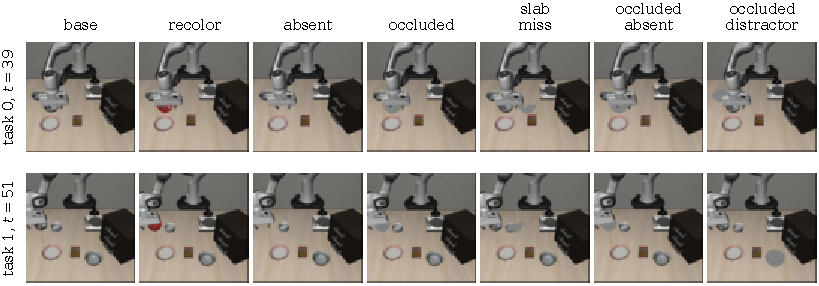
\includegraphics[width=\linewidth]{figures/fig_protocol.pdf}
  \caption{\textbf{Seven conditions}, shown as the policy sees them, for discovery frames of task 0 (top, demonstration) and task 1 (bottom, policy rollout). The target covers a median of 0.88\% of the agentview image and 8.0\% of the wrist image. \cond{occluded\_distractor} paints the identical second bowl.}
  \label{fig:protocol}
\end{figure}

\paragraph{Transcoders.} Each layer gets a TopK transcoder \citep{dunefsky2024transcoders,gao2025scaling},
$\vf(\vx)=\mathrm{TopK}_k(\mathrm{ReLU}(\mW_{\text{enc}}(\vx-\boldsymbol\mu_x)/s_x+\vb_{\text{enc}}))$ and $\hat\vy=s_y(\mW_{\text{dec}}^\top\vf+\vb_{\text{dec}})+\boldsymbol\mu_y$.
It has 2,048 features, $k{=}32$ and unit-norm decoder rows $\vd_j$. Inputs and outputs are normalized to unit mean norm, so the loss equals the fraction of variance unexplained (FVU).
\begin{itemize}[leftmargin=*,itemsep=0pt,topsep=1pt]
  \item \textbf{Training.} AuxK revival, Adam at $2{\times}10^{-3}$, batch 1,024 and 4,000 steps. A layer with FVU $>0.2$ is retrained once with 8,000 steps.
  \item \textbf{Data.} 146,599 valid prefix tokens from 258 forward passes on \emph{non-test} demonstrations: 20 discovery frames $\times$ 7 conditions plus the extra frames. 10\% of tokens are held out.
  \item \textbf{Out-of-sample checks.} We measure FVU and a splice test (replace the MLP by its reconstruction and measure the action change) on held-out test frames.
\end{itemize}

\paragraph{Selecting occlusion features (discovery frames only).} Let $\Delta_j(c)$ be feature $j$'s activation summed over valid tokens under condition $c$, minus its value under \cond{base}. A feature is \emph{occlusion-selective} if it meets three conditions:
\begin{enumerate}[leftmargin=*,itemsep=0pt,topsep=1pt,label=(\roman*)]
  \item $\Delta_j(\occ)>0$ on $\ge$90\% of discovery frames;
  \item its specificity $1-\max_c\overline{|\Delta_j(c)|}/\overline{\Delta_j(\occ)}$ is at least 0.5, for $c\in\{\cond{recolor},\cond{absent},\cond{slab\_miss}\}$;
  \item its rise $\overline{\Delta_j(\occ)}$ exceeds one typical token-level firing.
\end{enumerate}
It is \emph{target-specific} if (ii) still holds with \cond{occluded\_distractor} added to the quiet set. We keep up to 8 per layer, ranked by specificity$\times$rise, and also test the uncapped set. A \emph{colour} set is ranked the same way with \cond{recolor} as the target, with the same number of features per layer and at least one per layer.

\paragraph{Causal patching (test frames only).} Setting a feature set $S$ to its values from a target run edits the MLP output as $\vy'_\ell=\vy_\ell+s_y\sum_{j\in S}(f^{\text{tgt}}_j-f_j(\vx_\ell))\vd_j$. This keeps the transcoder error, so the patch is an exact edit along the dictionary directions.
\begin{itemize}[leftmargin=*,itemsep=1pt,topsep=2pt]
  \item \textbf{Primary site.} All 18 layers at once, on all valid tokens, fixed in advance.
  \item \textbf{Pass criterion.} The occlusion set must close at least 10 points more than both the norm-matched random control and the colour control.
  \item \textbf{Controls:} 10 random sets of $|S|$ features rescaled per token to the norm of the $S$ edit, 2 raw random sets, the colour set, all transcoder features, and the MLP-output swap $\vy_\ell\leftarrow\vy^{\text{occ}}_\ell$ (the ceiling of any edit at the site).
  \item \textbf{Further measurements:} bowl-token versus other-token scopes, the remove direction, the top-3 Goal-1 layers individually, single features, and cross-layer edges.
  \item \textbf{$k$-curve.} We patch the top-$K$ features ranked three ways: by each frame's own activation change $s_y\sum_t|f^{\text{occ}}_{j,t}-f^{\text{base}}_{j,t}|$, by the same quantity averaged over discovery frames, or at random.
  \item \textbf{Held-out replication.} We recompute the selection rule on the test frames from summed activations under all seven conditions.
\end{itemize}
Test frames with $g<0.1$ are excluded from patching, a rule fixed before the run.

\paragraph{Statistics and pre-specification.} CIs are 95\% percentile bootstraps that resample \emph{tasks} (10,000 draws). Goal-2 $p$-values are one-sided sign-flip tests over task means (exact, $2^{10}$ patterns) and over frames (200,000 Monte Carlo draws). The target-vs-distractor sign test and the McNemar test are two-sided.

Before the v2 run, the plan fixed the validity checks (Table~\ref{tab:validity}), the Goal-1 rule and the Goal-2 rule; they were pre-specified, not registered. Three thresholds were adapted from the pilot to the larger design:
\begin{itemize}[leftmargin=*,itemsep=0pt,topsep=1pt]
  \item check 3: the gap must reach 0.02 on $\ge$90\% of frames instead of all;
  \item the residual-swap ceiling: $\ge$80\% instead of 90\%;
  \item Goal-1 positivity: $\ge$90\% of frames instead of all.
\end{itemize}
Under the pilot's strict rules check 4 would still pass, check 3 would fail on one frame (gap 0.015, excluded from Goal 2 anyway), and Goal 1 would keep 14 of the 29 features. Q3 was gated on Q2. It is run here only as an explicitly exploratory check.

\section{Results}
\label{sec:results}

\paragraph{Run.} One process ran all steps on one A100 in 123 minutes. The dataset archive held demonstrations only for task 0, so tasks 1--9 used 45 policy rollouts under the same role mapping. 7 of these rollouts failed, and 8 probe frames come from them; \S\ref{sec:q2} shows the null without them.

\subsection{The instrument is sound}
\label{sec:validity}

\begin{table}[t]
\caption{\textbf{Validity battery} (60 probe frames; checks 2 and 4 on 8 frames spread over tasks). All checks pass.}
\label{tab:validity}
\centering\small
\resizebox{\linewidth}{!}{%
\begin{tabular}{@{}lll@{}}
\toprule
Check & Criterion & Result \\
\midrule
1. Edits are clean & $<0.2\%$ pixels changed outside edit region & 0.000\% (720 image checks); state \& prompt identical \\
2. Determinism & repeated forward pass, max $|\Delta\va|=0$ & 0.0 \\
3. Signal exists & gap $\ge0.02$ on $\ge$90\% of frames & 98\% of frames; median 0.186, 2.1$\times$ sampling noise \\
4. Ceiling works & residual swap $\ge80\%$ at some layer & 97.1\% at layer 1 (per frame 96.4--98.5\%) \\
5. Transcoders faithful & median held-out FVU $\le0.20$ & 0.185 (held-out \emph{test frames}: 0.400) \\
\bottomrule
\end{tabular}}
\end{table}

Table~\ref{tab:validity} shows that all five checks pass, and check~4 also clears the pilot's 90\% bar.

\paragraph{How the action responds to each edit.} Median action RMSE versus base, over 60 frames:
\begin{itemize}[leftmargin=*,itemsep=0pt,topsep=1pt]
  \item \cond{absent} moves the action most (0.649), a median $2.8\times$ the paint;
  \item \occ{} moves it by 0.186 and \cond{recolor} by 0.136;
  \item \cond{occluded\_distractor} moves it by 0.084.
\end{itemize}
The action responds to \emph{which} bowl is painted. Painting the target changes it more than painting the identical distractor on 44 of 60 frames, with a median ratio of $2.5\times$ (Figure~\ref{fig:heldout}b). The frame-level sign test gives $p{=}0.0004$. At the task level the target dominates in 8 of 10 tasks (two-sided $p{=}0.11$), and task 3 goes the other way on all of its frames.

\paragraph{Transcoder fit out of sample.} The transcoders generalize poorly to held-out frames. Test-frame FVU is a median $1.9\times$ the held-out-token FVU. Splicing a mid-layer transcoder (layers 1--13) moves the test-frame action by a median 0.82 of the gap, and by more than the gap in 4 layers. Our patches keep the error term, so they remain exact. The limited fit bounds how much of the MLP computation the dictionary can express.

\paragraph{Where the signal lives.} A full residual swap at one layer closes $\ge$90\% of the gap up to layer 7, falls below 50\% from layer 10 and below 5\% from layer 14 (Figure~\ref{fig:layers}a). At layer 17 it closes exactly 0\%: the expert reads per-layer keys and values, so the last layer's output never reaches it. A single layer's MLP output closes at most 22.1\% (layer 12).

\begin{figure}[t]
  \centering
  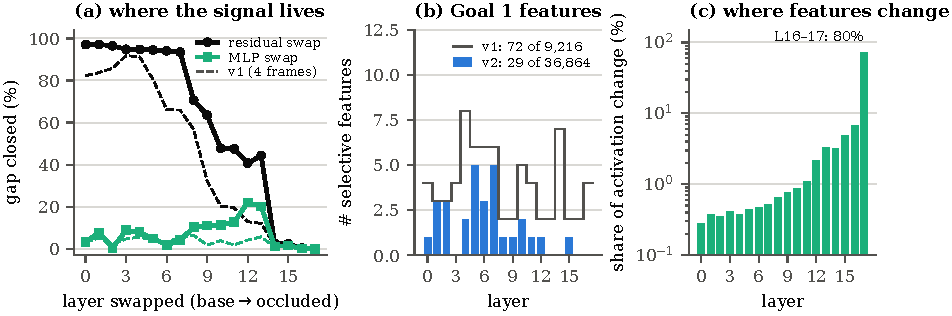
\includegraphics[width=\linewidth]{figures/fig_layers.pdf}
  \caption{\textbf{Layer profile.} (a) Gap closed by swapping a layer's full residual output (ink) or only its MLP output (aqua) with the occluded run's. Dashed lines: the pilot on 4 selected frames. (b) Occlusion-selective features per layer. (c) Share of the occlusion-induced activation change $s_y\sum_t|\Delta f|$ carried by each layer on discovery frames, log scale. 73\% is in layer 17, whose output cannot reach the action expert, and 7\% in layer 16, which barely can.}
  \label{fig:layers}
\end{figure}

\subsection{Q1: Selective, target-specific features exist and partly replicate}
\label{sec:q1}
Of 36,864 features, 29 (0.08\%) pass the rule on discovery frames, from 13 layers with at most 5 per layer (Figure~\ref{fig:layers}b). The per-layer cap therefore never binds. All 29 are also target-specific on discovery frames, so the capped, uncapped and target-specific sets coincide.
\begin{itemize}[leftmargin=*,itemsep=0pt,topsep=1pt]
  \item \textbf{Selectivity.} Median specificity is 0.64 (0.50--0.89) and median rise 29.0 token-firings. Relative to the occlusion response, the median responses are 0.20 to \cond{recolor}, 0.16 to \cond{absent}, 0.09 to \cond{slab\_miss} and 0.03 to \cond{occluded\_distractor}.
  \item \textbf{Paint versus object.} The features respond equally to paint with no bowl underneath: $r{=}0.9975$ between $\Delta(\occ)$ and $\Delta(\cond{occluded\_absent})$. They are ``flat patch where the \emph{target} is'' detectors. \pifive{} conditions on one frame, so object permanence is out of reach here \citep{baillargeon1985object}.
\end{itemize}

\textbf{Replication on held-out frames} (Figure~\ref{fig:heldout}a):
\begin{itemize}[leftmargin=*,itemsep=0pt,topsep=1pt]
  \item Recomputed on the 40 test frames, the full rule is passed by 8 of the 29 selected features (21 fail) and by none of the random or colour features.
  \item Only 12 of 36,802 live features pass on test frames, a base rate of 0.03\%. The selection is therefore enriched $846\times$, and 8 of those 12 features are ours.
  \item Across all live features, discovery and test occlusion responses correlate at Spearman $\rho{=}0.65$ (Pearson 0.80).
  \item On test frames the selected features keep a median specificity of 0.66 and a median distractor/target ratio of 0.058. Two of them are not target-specific there (ratios 0.51 and 0.44).
\end{itemize}
The selection captures a real, partly reproducible and largely target-selective signal. Replication is across demonstrations of the same tasks.

\begin{figure}[t]
  \centering
  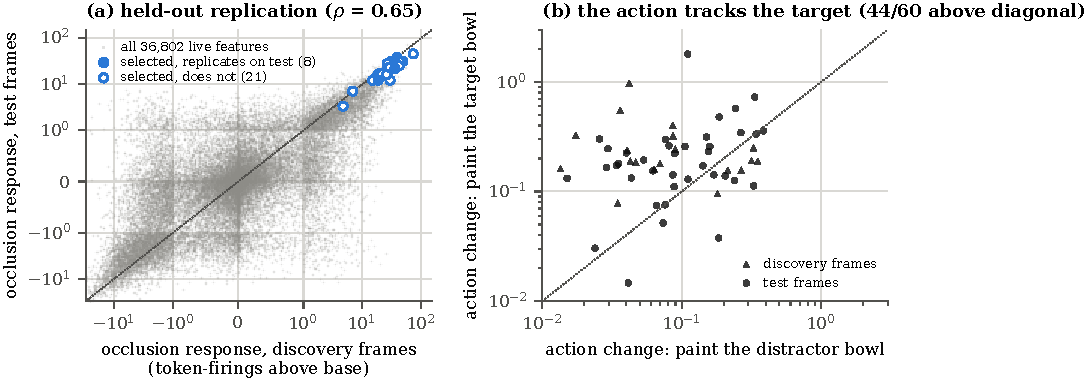
\includegraphics[width=\linewidth]{figures/fig_heldout.pdf}
  \caption{\textbf{Replication and target specificity.} (a) Occlusion response of every live feature on discovery vs.\ held-out test frames (token-firings, symmetric log). Selected features are blue; filled ones pass the full selection rule again on test frames. (b) Action change from painting the target vs.\ the identical distractor bowl, per frame.}
  \label{fig:heldout}
\end{figure}

\subsection{Q2: The features do not drive the action}
\label{sec:q2}

\begin{table}[t]
\caption{\textbf{Goal 2 on held-out test frames}: gap closed (\%) when patching base$\rightarrow$occluded at all 18 layers (34 frames with $g\ge0.1$, 10 tasks). CIs are 95\% task-clustered bootstrap intervals.}
\label{tab:goal2}
\centering\small
\begin{tabular}{@{}lrr@{}}
\toprule
Patch (inject, all valid tokens) & Gap closed (\%) & 95\% CI \\
\midrule
Occlusion features (29; $=$ uncapped $=$ target-specific) & \textbf{0.27} & [$-$0.32, 0.92] \\
Random, same norm (10 draws) & 0.05 & [$-$0.01, 0.11] \\
Random, raw (2 draws) & 0.05 & [$-$0.11, 0.20] \\
Colour features (34) & 0.05 & [$-$0.10, 0.17] \\
\midrule
All 36,864 transcoder features & 42.77 & [35.94, 50.64] \\
MLP-output swap (ceiling) & 76.61 & [68.51, 84.78] \\
\bottomrule
\end{tabular}
\end{table}

\begin{figure}[t]
  \centering
  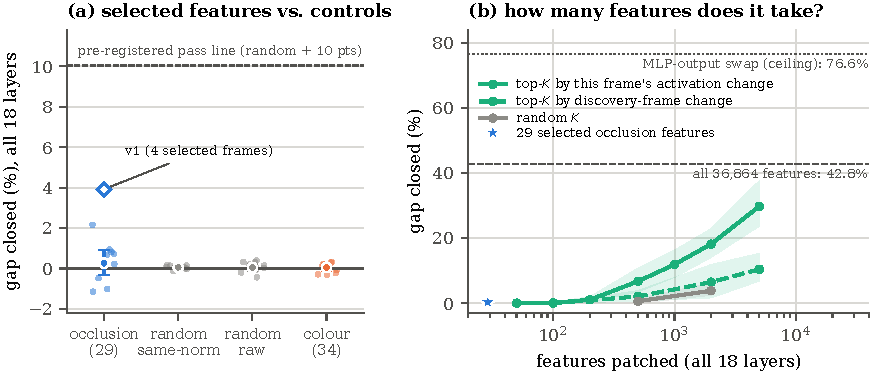
\includegraphics[width=\linewidth]{figures/fig_goal2.pdf}
  \caption{\textbf{Causal tests on held-out frames.} (a) Gap closed by the selected occlusion features and the controls at all 18 layers. Small dots are task means; large dots with bars are the mean and 95\% task-clustered CI. The dashed line is the pre-specified pass line, and the hollow diamond is the in-sample pilot. (b) Gap closed by the top-$K$ features, ranked by each frame's own activation change (solid aqua) or by discovery frames (dashed), or chosen at random (gray). The selected 29 are the star. Reference lines show all features and the MLP ceiling.}
  \label{fig:goal2}
\end{figure}

Table~\ref{tab:goal2} and Figure~\ref{fig:goal2}a show the result.
\begin{itemize}[leftmargin=*,itemsep=1pt,topsep=2pt]
  \item \textbf{Main result.} The 29 features close 0.27\% of the gap. The difference from same-norm random features is $+0.21$ points [$-0.35$, $+0.84$], with $p{=}0.222$ over tasks and $p{=}0.25$ over frames, and it is positive in 7 of 10 tasks. Against the colour set the difference is $+0.22$ [$-0.39$, $+0.86$].
  \item \textbf{Larger but inconsistent per-frame effects.} Per frame, the features move the action more than random features do: median $|$gap closed$|$ is 0.75 vs.\ 0.22 points. The sign is inconsistent: they beat every random draw on 12 of 34 frames, and lose to every draw on 8. They perturb the action, but not systematically toward the occluded action.
  \item \textbf{Verdict.} The margin is $+0.21$ against the required $+10$, so Goal 2 fails. The CI's upper bound is $12\times$ below the threshold, so this is not a power problem. The features carry 0.35\% of the MLP ceiling and 0.62\% of what all transcoder features carry.
\end{itemize}

\textbf{Every other test agrees:}
\begin{itemize}[leftmargin=*,itemsep=0pt,topsep=1pt]
  \item \emph{Single layers.} At the top Goal-1 layers the occlusion set closes $-0.03$\% (L5), $-0.07$\% (L1) and 0.11\% (L7), against site ceilings of 12.5--13.4\%.
  \item \emph{Single features.} The best single feature, L5~f93, closes 0.12\% [0.03, 0.21].
  \item \emph{Remove direction.} Restoring the features in the occluded run recovers 0.51\% [$-1.95$, 3.51], against 88.0\% for restoring all MLP outputs.
  \item \emph{Token scope.} Most of the MLP-mediated effect is off the painted patches: the MLP ceiling is 61.4\% on non-bowl tokens and 26.7\% on bowl tokens.
  \item \emph{Edges.} Injecting the L5 set activates 2.4\% of the L7 set's occlusion response (random: 0.3\%), a weak serial link.
\end{itemize}

\textbf{Robustness.} The null holds in every subset tested, and no upper CI bound on the difference from random exceeds 1.7 points (Appendix Table~\ref{tab:robust}). Subsets: without the 3 patched test frames from failed rollouts ($+0.15$ [$-0.48$, $+0.83$]), rollout tasks only, frames with $g\ge0.2$, and task 0 alone, the pilot's task ($-1.02$\%).

\subsection{The effect is distributed, and magnitude is a poor guide}
\label{sec:dist}
The $k$-curve (Figure~\ref{fig:goal2}b) shows how many features the occlusion effect takes.
\begin{itemize}[leftmargin=*,itemsep=1pt,topsep=2pt]
  \item \textbf{Per-frame ranking.} Ranked by each frame's own activation change, the top 500 features close 6.71\%, the top 2,000 18.18\% and the top 5,000 29.80\%. The top 5,000 are 14\% of the dictionary and reach 70\% of the all-feature effect. This ranking beats random $K$ by $11\times$ at $K{=}500$ and $4.7\times$ at $K{=}2{,}000$.
  \item \textbf{Transfer.} The discovery-frame ranking transfers only partly: 10.45\% at $K{=}5{,}000$ and $1.7\times$ random at $K{=}2{,}000$.
  \item \textbf{Magnitude is misleading.} Half of each frame's activation change sits in a median of 35.5 features, yet the top 50 close just 0.02\%.
  \begin{itemize}[leftmargin=*,itemsep=0pt,topsep=0pt]
    \item The reason is where the change lives. On discovery frames, 80\% of it is in layers 16--17 (Figure~\ref{fig:layers}c), where the MLP output's RMS norm $s_y$ reaches 1,608 and 7,697, against 36--71 in layers 1--10. A proxy from the saved test-frame sums puts a median 100\% of each frame's top 50 there as well.
    \item Layer 17 is inert for the action: its output never reaches the expert, and splicing it changes nothing. Layer 16 is nearly inert, with a residual swap of 0.4\%.
  \end{itemize}
  \item \textbf{The selected features.} They lie in the top 13\% of features by activation change, but none is among any frame's top 29.
\end{itemize}
Feature rankings in VLAs should therefore be causal (attribution-based) and restricted to layers whose outputs reach the action expert.

\subsection{Q3 (exploratory): closed loop}
\label{sec:q3}
On task 0 with 10 initial states, success is identical with and without the target painted in both cameras on every step (0.9 and 0.9). A likely reason is visible in the recorded episode: the paint keeps the bowl's silhouette, and the robot grasps the gray blob (Appendix Figure~\ref{fig:loop}). Ablating the 29 features at their 13 layers, or amplifying them $3\times$, gives 0.8 each. Each difference comes from a single discordant episode (paired CI [$-0.30$, 0.00]; McNemar $p{=}1.0$). With 10 episodes we detect no shift from either the features or this form of occlusion; only large effects would be visible.

\subsection{Pilot (in-sample) vs.\ held-out protocol}
\label{sec:compare}

\begin{table}[t]
\caption{\textbf{In-sample pilot (v1) vs.\ held-out protocol (v2)}: same model, questions, gap metric and 10-point rule. Gap closed (\%) at the all-layer site. The pilot had no CI with 4 frames.}
\label{tab:compare}
\centering\small
\resizebox{\linewidth}{!}{%
\begin{tabular}{@{}lll@{}}
\toprule
 & v1: in-sample pilot & v2: held-out (this paper) \\
\midrule
Tasks / probe frames & 1 / 4 & 10 / 60 (20 discovery, 40 test) \\
Frame choice & largest gap of 8 candidates & fixed phases 0.4, 0.8 \\
Selection vs.\ test frames & same & disjoint demonstrations \\
Transcoders (features, $k$, training tokens) & 512, 16, 26,852 incl.\ test frames & 2,048, 32, 146,599 discovery only \\
Median FVU: held-out tokens / test frames & 0.174 / not measured & 0.185 / 0.400 \\
Best residual swap / max single-layer MLP swap & 91.8\% (L3) / 6.5\% & 97.1\% (L1) / 22.1\% \\
Selective features & 72 of 9,216 (0.78\%) & 29 of 36,864 (0.08\%), all target-specific \\
Held-out replication & -- & 8 of 29 ($846\times$ base rate); $\rho{=}0.65$ \\
Occlusion features & 3.92 & 0.27 [$-$0.32, 0.92] \\
Random (same norm) / colour & 0.56 / 0.66 & 0.05 / 0.05 \\
Occlusion / random ratio & $6.9\times$ & $4.9\times$ (difference n.s.) \\
Share of dictionary patched & 0.78\% & 0.08\% \\
Margin (+10 needed); $p$ & $+3.26$; 0.125 (4 frames) & $+0.21$; 0.222 (10 tasks) \\
All transcoder features / MLP ceiling & 40.1 / 65.5 & 42.8 / 76.6 \\
Occlusion share of ceiling & 6.0\% & 0.35\% \\
Remove: occlusion features / MLP swap & 7.9 / 85.6 & 0.51 / 88.0 \\
Closed loop & not run & exploratory: 0.9 / 0.9 / 0.8 / 0.8 \\
\bottomrule
\end{tabular}}
\end{table}

Table~\ref{tab:compare} sets the pilot beside the held-out run.
\begin{itemize}[leftmargin=*,itemsep=1pt,topsep=2pt]
  \item \textbf{What held up.} The validity battery improved, and sparse selective features exist in both runs. The all-feature effect (40.1 and 42.8\%) and the MLP ceiling (65.5 and 76.6\%) are similar, as is a weak serial edge between two Goal-1 layers (2.3 and 2.4\%).
  \item \textbf{What did not.} The pilot's reading that the selected features act above chance. Its $6.9\times$ ratio over random ($p{=}0.125$ on 4 selected frames) becomes $4.9\times$, with a paired difference of $+0.21$ [$-0.35$, $+0.84$]. On the pilot's own task, held-out frames give $-1.02$\%.
  \item \textbf{What is not comparable.} Absolute effects. The selected set fell from 3.92\% to 0.27\% ($15\times$), but the random and colour controls fell $10\times$ and $14\times$, because v2 patches a tenth of v1's share of a $4\times$ wider dictionary.
\end{itemize}
The pilot's design (frames chosen by effect size, features tested where they were selected) is a known source of inflation \citep{kriegeskorte2009circular}. The runs also differ in dictionary and set size, so these data cannot attribute the change to any single factor.

\section{Discussion}
\label{sec:discussion}
\paragraph{Existence is not mechanism.} Sparse, partly reproducible, target-selective features in a VLA can have a negligible net causal effect. Held-out replication and held-out causal tests answer different questions, and both are needed before a feature is called a mechanism. Our selection criteria (positivity, specificity, rise) find what the model \emph{notices}, not what it \emph{uses}.

\paragraph{Why the effect is distributed.} The edit changes pixels in both cameras, and bidirectional attention spreads it to every token whose keys and values the expert reads; the residual swap shows the usable signal is present by layers 1--7. No single MLP site is a bottleneck ($\le$22\% each, 77\% together). This complements reports that vision pathways dominate \pifive{}'s actions \citep{grant2026features}; the attention-level bottlenecks of \citet{shi2026vlatrace} concern routing, not feature sparsity.

\paragraph{Practical recommendations.} (1) Select on discovery data, test on disjoint data, and report task-clustered CIs. (2) Report each site's ceiling and a $k$-curve, not a single selected set. (3) Rank features by attribution, only within layers that can reach the action head. (4) Include distractor controls that separate ``the target'' from ``an object of that kind''.

\section{Limitations}
\label{sec:limitations}
\begin{itemize}[leftmargin=*,itemsep=1pt,topsep=2pt]
  \item \textbf{Frame sources.} Only task 0 had demonstrations, so 9 tasks use policy rollouts, 7 of which failed. Dropping the 3 patched test frames from failed rollouts does not change the result, but two discovery frames and some training frames from them remain, and five test frames show no target in the wrist camera.
  \item \textbf{Replication scope.} Held-out frames come from the same 10 tasks, so replication across tasks is untested.
  \item \textbf{Transcoder fidelity.} Transcoders trained on about 138 scenes fit held-out frames poorly (FVU 0.40). A better dictionary, for example cross-layer transcoders \citep{ameisen2025circuit} or residual SAEs at layers 1--7, might represent the effect with fewer features.
  \item \textbf{The occluder.} It is flat paint that preserves the silhouette. \pifive{} has no memory, so object permanence cannot be tested.
  \item \textbf{Rankings.} The $k$-curve ranks by magnitude, not attribution, so it upper-bounds how many features are needed.
  \item \textbf{Scope.} One policy and one suite. Q3 uses one task and 10 episodes per condition, so it detects only large shifts.
\end{itemize}

\section{Conclusion}
Under a held-out protocol, \pifive{} contains selective, largely target-specific and partly reproducible occlusion features whose net effect on its actions is negligible: the CI excludes the pre-specified effect by an order of magnitude. The occlusion signal runs through many MLP features and the full residual stream, and an in-sample pilot's above-chance effect does not survive held-out testing. Held-out selection and testing should be standard for circuit claims about robot policies.

\subsubsection*{AI use statement}
% AUTHORS: review and edit this statement so that it accurately reflects your process before submission.
Generative AI tools (a large language model assistant) were used to write and debug the experimental pipeline code (rendering, hooks, transcoder training, patching, statistics), to compute the derived statistics, to produce the summary figures, and to draft this manuscript. The research questions, the gated experimental plan and its thresholds were specified before the experiments were run. All reported numbers were cross-checked programmatically against the raw result files, and every cited work was checked against its public record. The authors reviewed all AI-assisted work and take full responsibility for the content of this paper.

\subsubsection*{Ethics statement}
This work analyzes a publicly released robot policy in simulation only and involves no human subjects or personal data. Understanding how VLAs treat hidden objects may help find unsafe failure modes before deployment.

\subsubsection*{Reproducibility statement}
Section~\ref{sec:method} and Appendix~\ref{app:repro} specify every hyper-parameter. The supplementary material contains:
\begin{itemize}[leftmargin=*,itemsep=0pt,topsep=1pt]
  \item the complete pipeline (one script with seven chainable subcommands), its configuration, the Colab notebook with all outputs, and the full run log;
  \item every raw result file, including all individual patching runs, per-feature statistics for the whole dictionary, per-frame feature sums on test frames, and closed-loop videos;
  \item scripts that regenerate every number and figure in this paper and check the quoted values against the data.
\end{itemize}

\bibliography{references}
\bibliographystyle{iclr2027_conference}

\appendix
\section{Reproducibility details}
\label{app:repro}
\paragraph{Software and hardware.} We used LeRobot 0.6.1, transformers 5.5.4, PyTorch 2.11.0 (CUDA 12.8), MuJoCo 3.8.1, robosuite 1.4.0, NumPy 2.2.6 and Python 3.12 on one NVIDIA A100-SXM4-80GB. Wall-clock time per step (one process, policy loaded once):
\begin{itemize}[leftmargin=*,itemsep=0pt,topsep=1pt]
  \item frames 41.3\,min, including 45 rollouts;
  \item validation 8.9\,min;
  \item capture 3.9\,min;
  \item transcoder training 11.1\,min;
  \item Goal 1 0.5\,min;
  \item Goal 2 28.0\,min;
  \item Goal 3 29.1\,min.
\end{itemize}

\paragraph{Implementation notes.}
\begin{itemize}[leftmargin=*,itemsep=0pt,topsep=1pt]
  \item \textbf{Model and simulator.} The checkpoint's \texttt{torch.compile} (CUDA graphs) bypasses hooks, so it is disabled. MuJoCo segmentation is decoded manually, because robosuite 1.4 overflows under NumPy 2.
  \item \textbf{Frames.} The lift is the first step at which the target rises 1\,cm above its initial height. 59 of 60 frames lie exactly at their nominal phase. Task 4's test rollouts never lifted the bowl, so their frames fall at $t{=}114$ and 223.
  \item \textbf{Bowl tokens.} These are SigLIP patches at least 10\% covered by paint, after the LIBERO $180^\circ$ flip.
  \item \textbf{Transcoder training.} Learning-rate warm-up over 5\% of steps and linear decay over the last 20\%. AuxK uses $k_{\text{aux}}{=}64$ and weight 1/32, and a feature counts as dead after 50 steps without firing.
  \item \textbf{Retraining.} Layers 6 and 8--12 exceeded FVU 0.2 and were retrained with 8,000 steps. Each improved by about 0.003 and stayed above 0.2.
  \item \textbf{Closed loop.} The Goal-3 patches multiply the selected features by 0 or 3 on every valid prefix token at every inference step.
\end{itemize}

\paragraph{Deviations and disclosures.}
\begin{itemize}[leftmargin=*,itemsep=0pt,topsep=1pt]
  \item Demonstrations were available only for task 0, so tasks 1--9 used policy rollouts.
  \item Three thresholds were adapted from the pilot before the v2 run: check 3 (all frames $\rightarrow\ge$90\%), check 4 (90$\rightarrow$80\%) and Goal-1 positivity (all frames $\rightarrow\ge$90\%). Under the strict rules, check 3 fails on one frame, check 4 passes (97.1\%), and Goal 1 keeps 14 of 29 features.
  \item Goal 3 was run as exploratory although the Goal-2 gate failed.
\end{itemize}

\clearpage
\section{Additional results}

\begin{table}[h]
\caption{Robustness of the Goal-2 null (all 18 layers; gap closed \%, 95\% task-clustered CI).}
\label{tab:robust}
\centering\small
\begin{tabular}{@{}lcrr@{}}
\toprule
Subset of test frames & Frames / tasks & Occlusion features & Occlusion $-$ random \\
\midrule
All included ($g\ge0.1$) & 34 / 10 & 0.27 [$-$0.32, 0.92] & $+$0.21 [$-$0.35, 0.84] \\
Without frames from failed rollouts & 31 / 9 & 0.19 [$-$0.46, 0.91] & $+$0.15 [$-$0.48, 0.83] \\
Without the largest-gap frame & 33 / 10 & 0.27 [$-$0.33, 0.96] & $+$0.22 [$-$0.36, 0.87] \\
Rollout tasks 1--9 only & 30 / 9 & 0.44 [$-$0.15, 1.08] & $+$0.38 [$-$0.18, 0.98] \\
Gap $\ge0.2$ only & 18 / 9 & 0.61 [$-$0.24, 1.74] & $+$0.56 [$-$0.26, 1.68] \\
Task 0 only (demonstrations) & 4 / 1 & $-$1.02 & $-$1.03 \\
\bottomrule
\end{tabular}
\end{table}

\begin{table}[h]
\caption{Per-layer transcoder quality and single-layer swap ceilings (swaps: mean over 8 frames).}
\centering\small
\setlength{\tabcolsep}{3.0pt}
\resizebox{\linewidth}{!}{%
\begin{tabular}{@{}l*{18}{r}@{}}
\toprule
Layer & 0 & 1 & 2 & 3 & 4 & 5 & 6 & 7 & 8 & 9 & 10 & 11 & 12 & 13 & 14 & 15 & 16 & 17 \\
\midrule
FVU, held-out tokens & .021 & .162 & .167 & .183 & .187 & .176 & .220 & .178 & .223 & .227 & .290 & .228 & .237 & .188 & .170 & .187 & .023 & .039 \\
FVU, test frames & .073 & .501 & .404 & .432 & .404 & .353 & .489 & .349 & .430 & .414 & .521 & .396 & .468 & .325 & .267 & .306 & .032 & .053 \\
Splice / gap (test) & .27 & .70 & .57 & .94 & .97 & 1.02 & .82 & .78 & .81 & .78 & .81 & 1.07 & 1.22 & 1.15 & .33 & .28 & .08 & .00 \\
Residual swap (\%) & 97.1 & 97.1 & 96.5 & 94.8 & 94.7 & 94.5 & 94.1 & 93.4 & 70.6 & 63.5 & 47.8 & 47.5 & 40.7 & 44.3 & 2.7 & 2.4 & 0.4 & 0.0 \\
MLP swap (\%) & 3.3 & 7.8 & 0.5 & 8.8 & 7.9 & 5.0 & 1.8 & 4.1 & 10.3 & 11.1 & 11.3 & 12.7 & 22.1 & 20.1 & 1.2 & 1.5 & 0.2 & 0.0 \\
$s_y$ (MLP output scale) & 60 & 39 & 36 & 42 & 41 & 48 & 47 & 58 & 59 & 68 & 71 & 103 & 164 & 270 & 284 & 423 & 1608 & 7697 \\
\# selective & 1 & 3 & 3 & 0 & 2 & 5 & 3 & 5 & 1 & 1 & 2 & 1 & 1 & 0 & 0 & 1 & 0 & 0 \\
\bottomrule
\end{tabular}}
\end{table}

\begin{table}[h]
\caption{$k$-curve on held-out frames (all 18 layers; gap closed \%).}
\centering\small
\begin{tabular}{@{}lrrrrrrrr@{}}
\toprule
$K$ & 50 & 100 & 200 & 500 & 1,000 & 2,000 & 5,000 & 36,864 \\
\midrule
Top-$K$, per-frame activation change & 0.02 & 0.12 & 1.04 & 6.71 & 11.91 & 18.18 & 29.80 & 42.77 \\
Top-$K$, discovery-frame change & & 0.03 & & 2.07 & & 6.47 & 10.45 & \\
Random $K$ & & & & 0.61 & & 3.84 & & \\
\bottomrule
\end{tabular}
\end{table}

\begin{figure}[h]
  \centering
  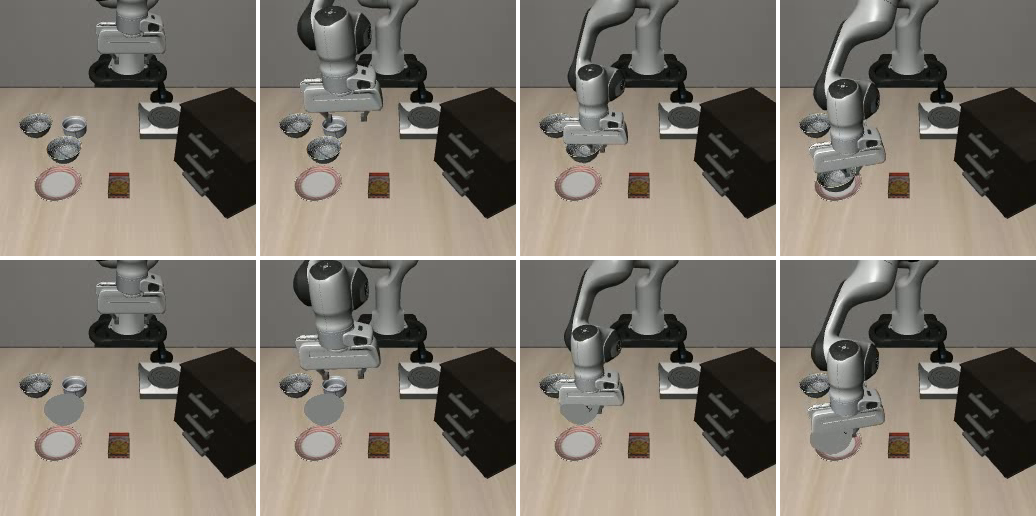
\includegraphics[width=0.92\linewidth]{figures/fig_closed_loop.png}
  \caption{Closed loop, task 0, episode 0: the clean reference (top) and the bowl painted in both cameras on every step (bottom). The paint keeps the bowl's silhouette, and the robot grasps the gray blob and places it on the plate.}
  \label{fig:loop}
\end{figure}

\begin{figure}[h]
  \centering
  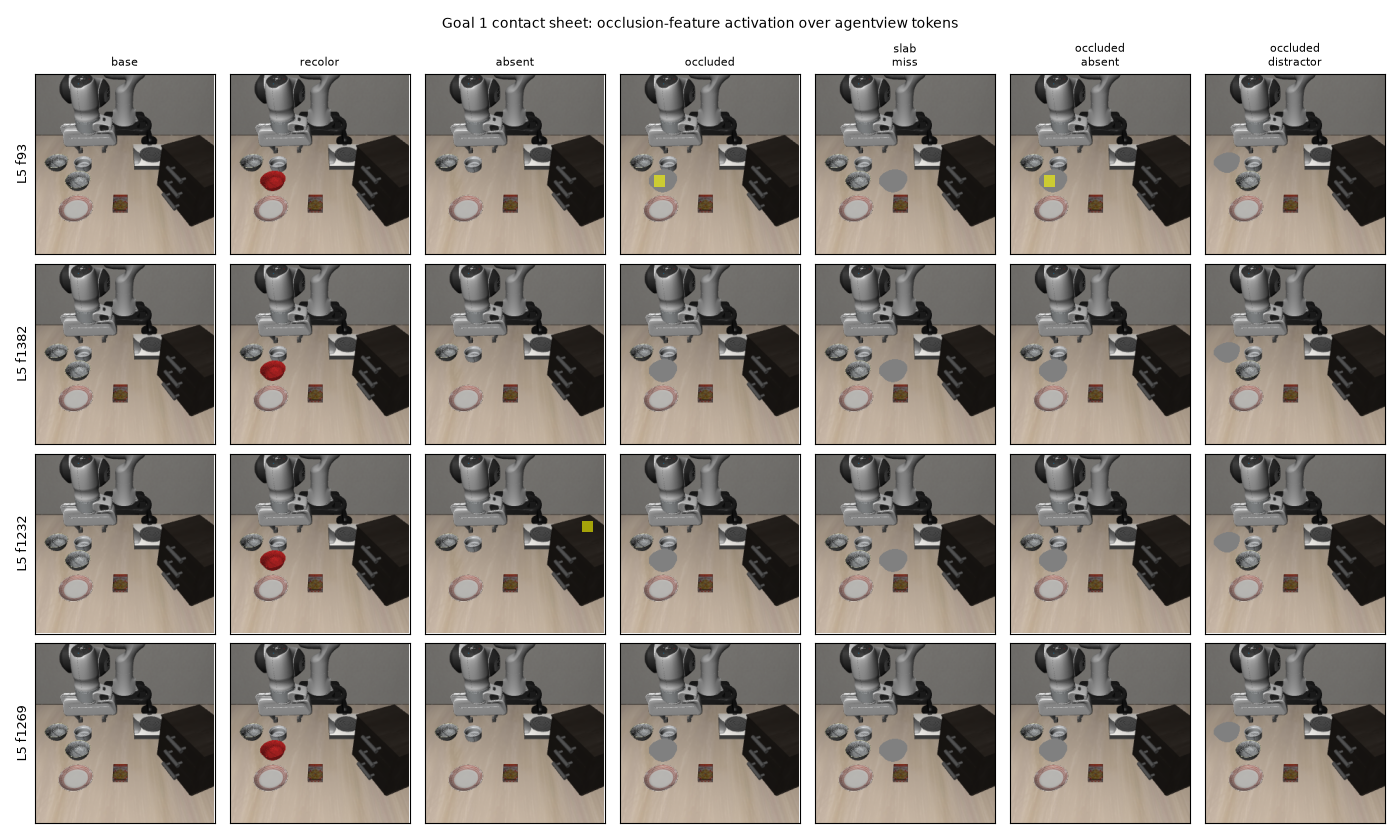
\includegraphics[width=0.92\linewidth]{figures/fig_goal1_contact_sheet.png}
  \caption{Activation maps of four layer-5 occlusion features over agentview tokens (discovery frame 0, task 0) for every condition. L5~f93 fires under the painted target and under \cond{occluded\_absent}, and not under the painted distractor. The other three show little agentview activation in this frame.}
\end{figure}

\begin{figure}[h]
  \centering
  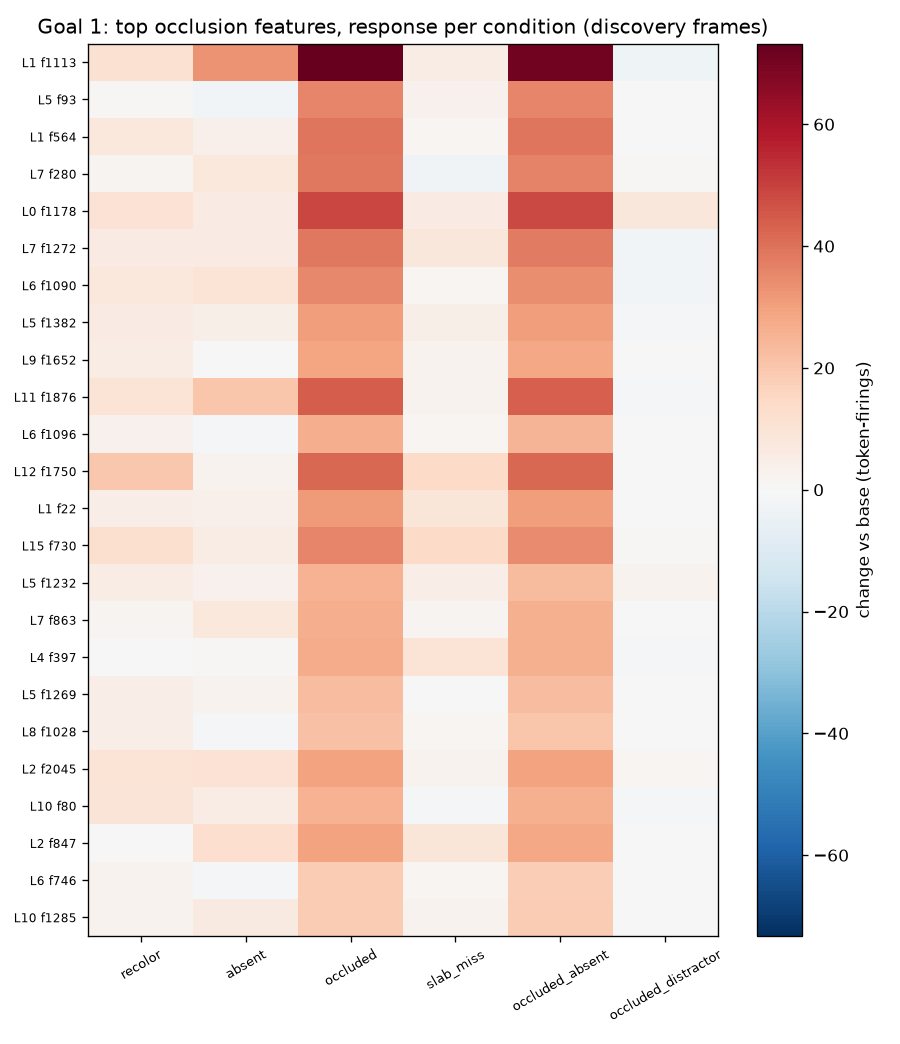
\includegraphics[width=0.6\linewidth]{figures/fig_goal1_features.png}
  \caption{Response of the 24 highest-scoring selected features to each condition on discovery frames (change vs.\ \cond{base}, token-firings). The \occ{} and \cond{occluded\_absent} columns match, and the \cond{occluded\_distractor} column is near zero.}
\end{figure}

\begin{figure}[h]
  \centering
  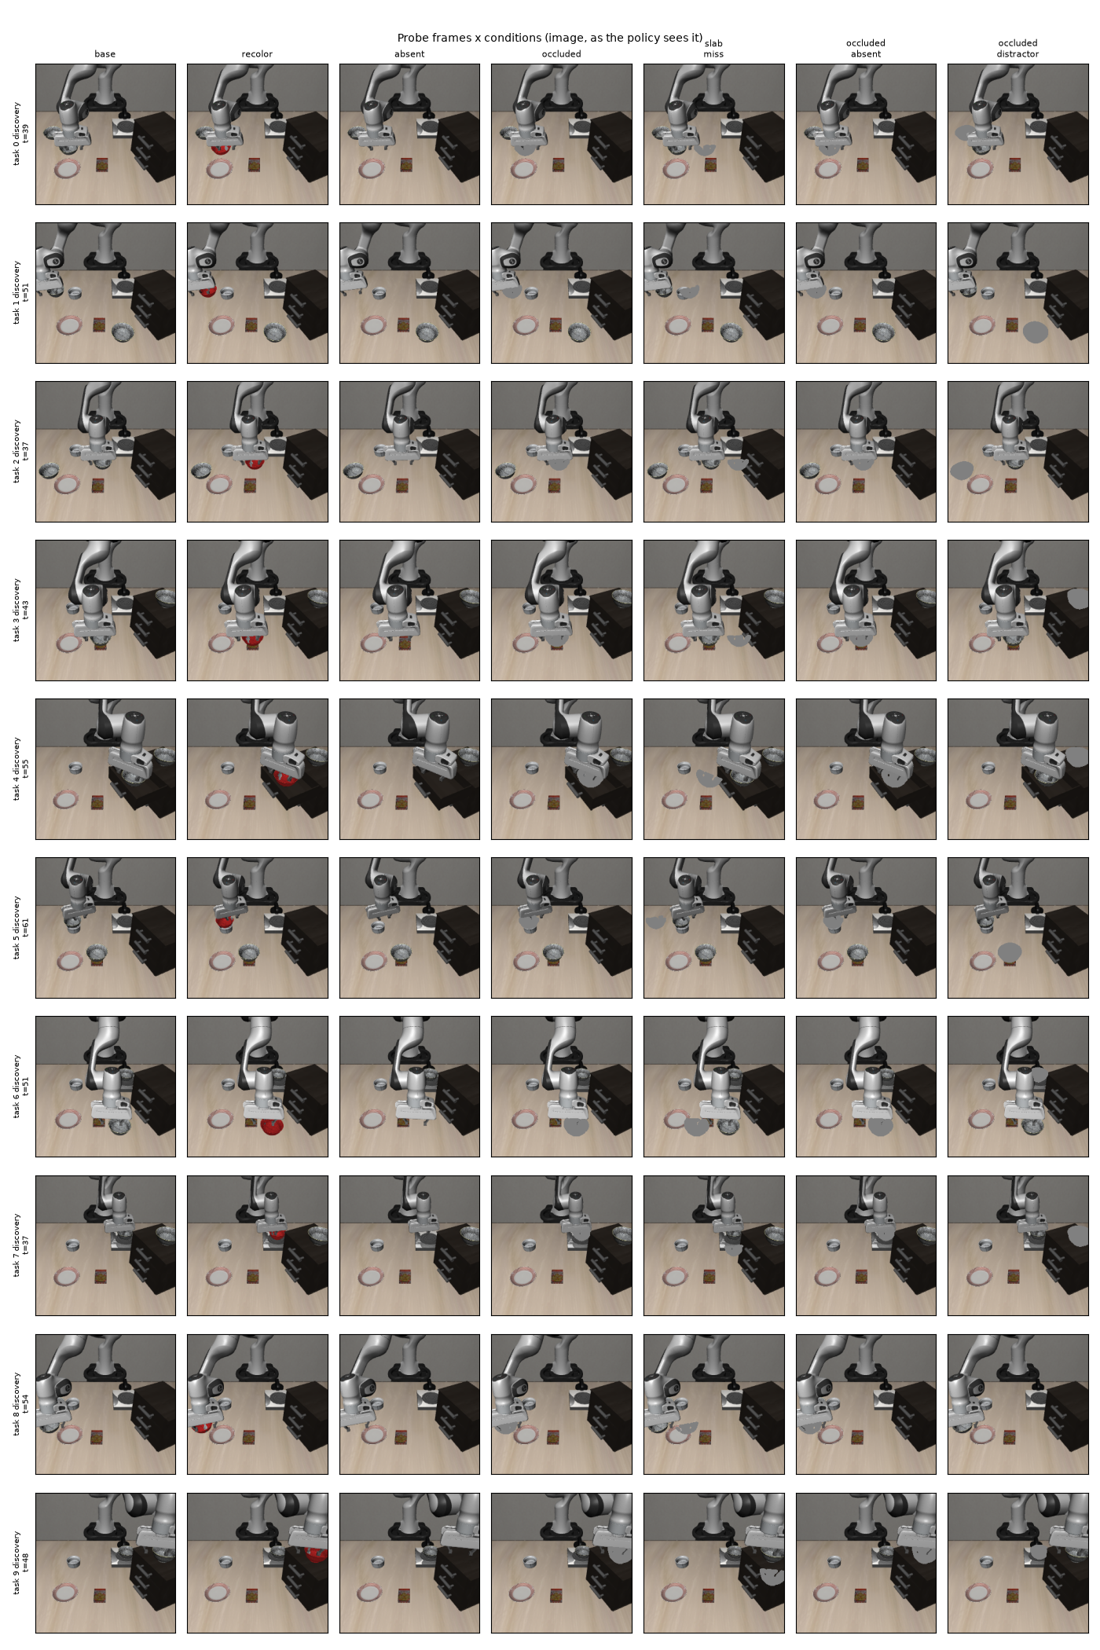
\includegraphics[width=0.9\linewidth]{figures/fig_probe_conditions_agentview.png}
  \caption{One discovery frame per task (rows: tasks 0--9) in all seven conditions, agentview camera.}
\end{figure}

\end{document}
